% Digital Logic Report Template
% Created: 2020-01-10, John Miller

%==========================================================
%=========== Document Setup  ==============================

% Formatting defined by class file
\documentclass[11pt]{article}

% ---- Document formatting ----
\usepackage[margin=1in]{geometry}	% Narrower margins
\usepackage{booktabs}				% Nice formatting of tables
\usepackage{graphicx}				% Ability to include graphics

%\setlength\parindent{0pt}	% Do not indent first line of paragraphs 
\usepackage[parfill]{parskip}		% Line space b/w paragraphs
%	parfill option prevents last line of pgrph from being fully justified

% Parskip package adds too much space around titles, fix with this
\RequirePackage{titlesec}
\titlespacing\section{0pt}{8pt plus 4pt minus 2pt}{3pt plus 2pt minus 2pt}
\titlespacing\subsection{0pt}{4pt plus 4pt minus 2pt}{-2pt plus 2pt minus 2pt}
\titlespacing\subsubsection{0pt}{2pt plus 4pt minus 2pt}{-6pt plus 2pt minus 2pt}

% ---- Hyperlinks ----
\usepackage[colorlinks=true,urlcolor=blue]{hyperref}	% For URL's. Automatically links internal references.

% ---- Code listings ----
\usepackage{listings} 					% Nice code layout and inclusion
\usepackage[usenames,dvipsnames]{xcolor}	% Colors (needs to be defined before using colors)

% Define custom colors for listings
\definecolor{listinggray}{gray}{0.98}		% Listings background color
\definecolor{rulegray}{gray}{0.7}			% Listings rule/frame color

% Style for Verilog
\lstdefinestyle{Verilog}{
	language=Verilog,					% Verilog
	backgroundcolor=\color{listinggray},	% light gray background
	rulecolor=\color{blue}, 			% blue frame lines
	frame=tb,							% lines above & below
	linewidth=\columnwidth, 			% set line width
	basicstyle=\small\ttfamily,	% basic font style that is used for the code	
	breaklines=true, 					% allow breaking across columns/pages
	tabsize=3,							% set tab size
	commentstyle=\color{gray},	% comments in italic 
	stringstyle=\upshape,				% strings are printed in normal font
	showspaces=false,					% don't underscore spaces
}

% How to use: \Verilog[listing_options]{file}
\newcommand{\Verilog}[2][]{%
	\lstinputlisting[style=Verilog,#1]{#2}
}


\usepackage[section]{placeins}

%======================================================
%=========== Body  ====================================
\begin{document}

\title{ELC 2137 Lab 8: 4-digit Display}
\author{Aaron Mendoza}

\maketitle


\section*{Summary}

The purpose of this lab is to build a 4-digit display that can switch between hexadecimal and BCD output using modules built in previous labs.

The modules that are used from previous labs are the eleven-bit BCD converter, the add3 module, and the seven-segment decoder. These will be used within the modules that were built in this lab. 

The first module I built in this lab was a 2-input MUX module. This works exactly like the MUX module built in previous labs: it has two inputs, a select input, and an output. However, when coding for this MUX, I used a parameter. Parameters are basically like constants in c++. Prior to listing the inputs in my module, I declared a paramter called BITS that corresponds with the number of bits that are in the input and output of the MUX. For example, the first MUX of this lab required 16 bits, so I set BITS equal to 16 and in my inputs I used [BITS-1:0] when declaring the size of the inputs and output. This use of paramters allows for flexible, reusable modules. 

The next module I built was a 4-input MUX module. The only difference with this MUX is that it has four inputs and the select is two bits rather than one. I used another parameter this time as well but set BITS equal to 4.

Following the mux4 module, I built a anode decoder module that decides which digit on the display will show. I used a case statement when coding this since the inputs were only two bits, so there were only four cases. The 0 case corresponds with the ones digit, and 1 case corresponds with the tens digit, and so on to the thousands digit.

The next module built was the four digit driver. This combines all of the previous modules into one single module. It had four inputs: 16 bits for data, 2 bits for digit select, one bit for hex or BCD, and one bit for the negative sign. The four outputs were the seven segment display, the decimal point, and the anode. This module was completely covered by a wrapper called sseg4 manual whose inputs and outputs corresponded with the constraints file of the Basys3 board. To check if my code was working properly, I added two simulation files that allowed me to check if my output matched the given output of the lab during the simulation of my top level module.

\section*{Results}

\begin{figure}[ht]\centering
		\caption{ERT for mux2 Module}
		\label{tbl:example_table}
		\begin{tabular}{ccc|c}
			\toprule
			in0 & in1 & sel & out \\
			\midrule
			000000000000001 & 111111111111110 & 0 & 000000000000001 \\
			000000000000001 & 111111111111110 & 1 & 111111111111110 \\
			101010101010101 & 000000000111111 & 0 & 101010101010101 \\
			101010101010101 & 000000000111111 & 1 & 000000000111111 \\
			\bottomrule
		\end{tabular} 
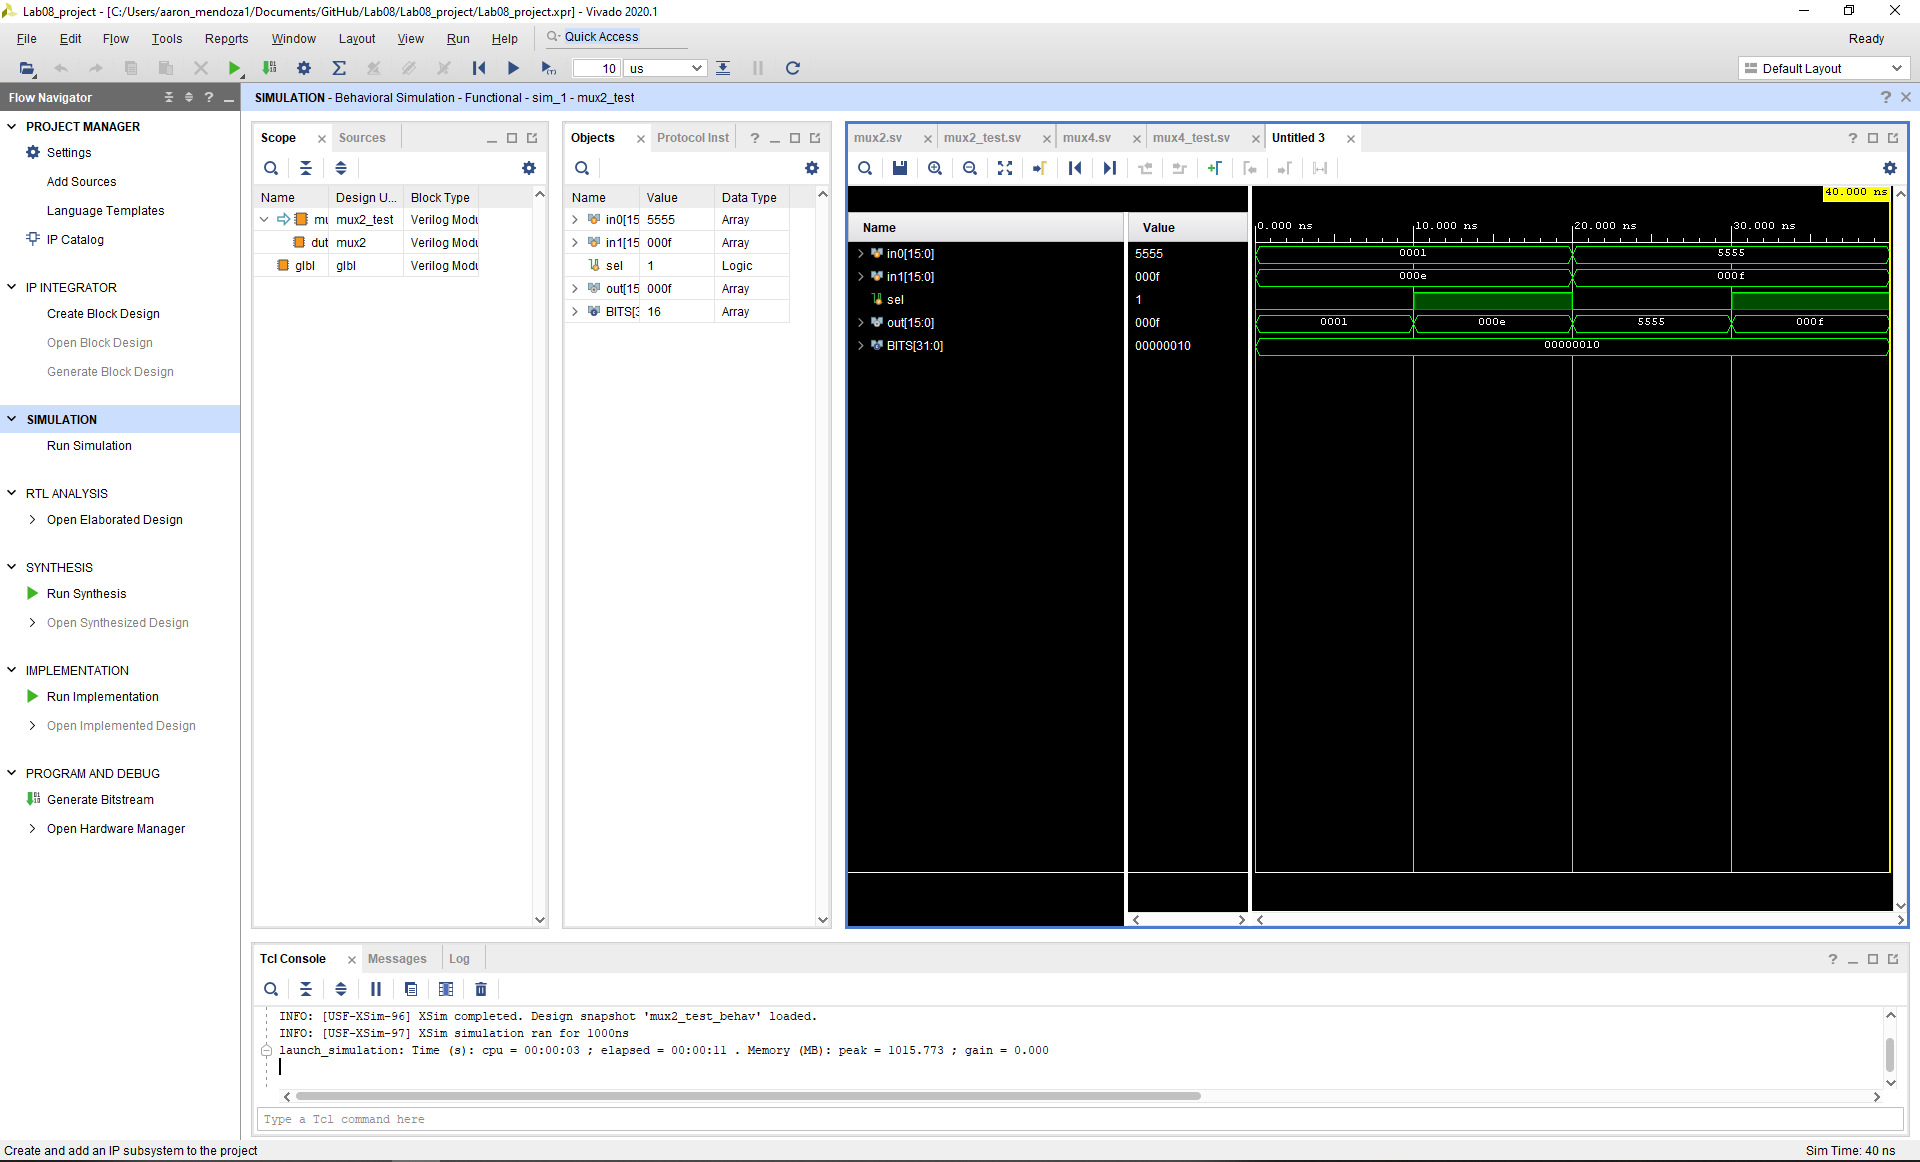
\includegraphics[width=1\textwidth,trim=19cm 15cm 0.5cm 4.5cm,clip]{mux2_test_screenshot}
	\caption{mux2 Simulation}
	\label{fig:sim_with_table}
\end{figure}

\FloatBarrier

\begin{figure}[ht]\centering
		\caption{ERT for mux4 Module}
		\label{tbl:example_table}
		\begin{tabular}{ccccc|c}
			\toprule
			in0 & in1 & in2 & in3 & sel & out \\
			\midrule
			0000 & 0001 & 0010 & 0011 & 00 & 0000 \\
			0000 & 0001 & 0010 & 0011 & 01 & 0001 \\
			0000 & 0001 & 0010 & 0011 & 10 & 0010 \\
			0000 & 0001 & 0010 & 0011 & 11 & 0011 \\
			0110 & 1111 & 1010 & 0101 & 00 & 0110 \\
			0110 & 1111 & 1010 & 0101 & 01 & 1111 \\
			0110 & 1111 & 1010 & 0101 & 10 & 0110 \\
			0110 & 1111 & 1010 & 0101 & 11 & 0101 \\
			\bottomrule
		\end{tabular} 
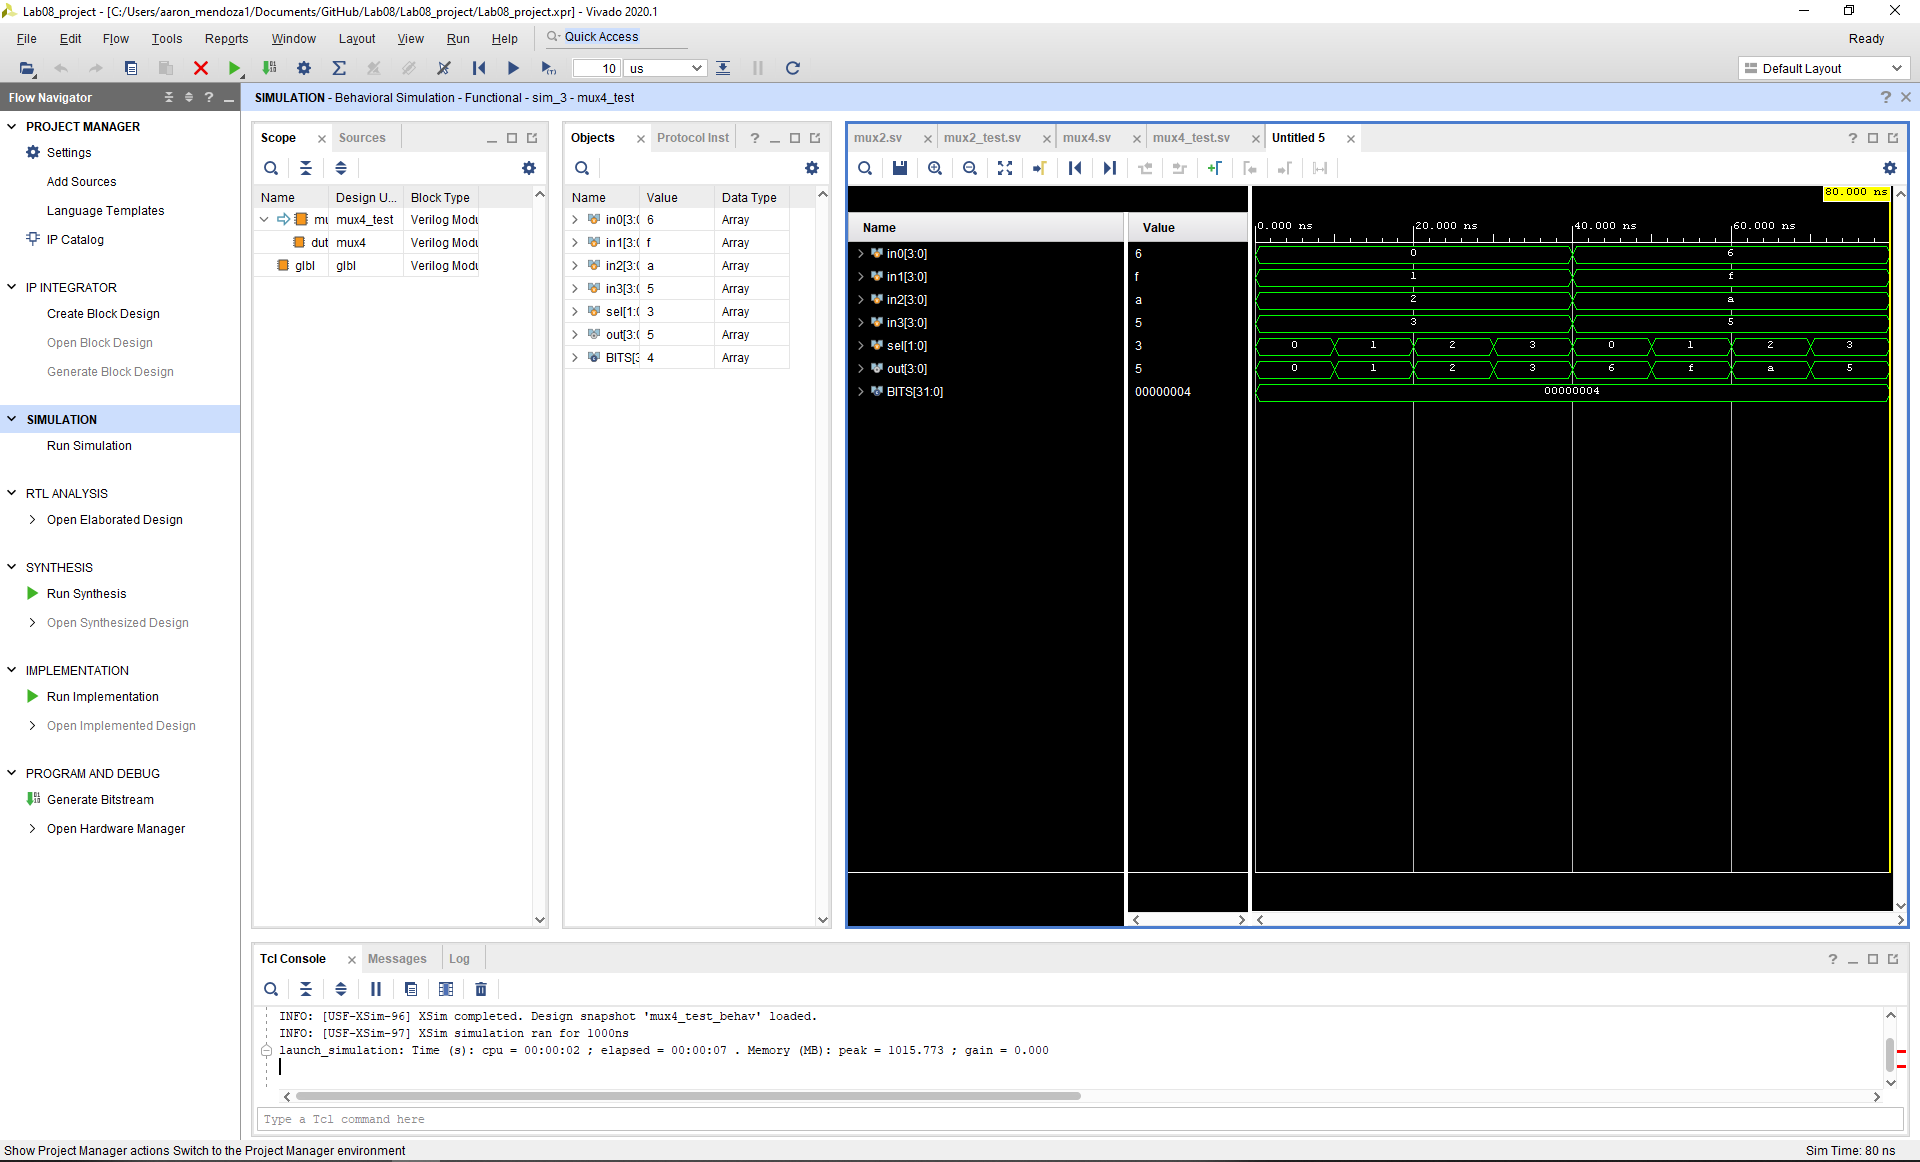
\includegraphics[width=1\textwidth,trim=19cm 15cm 0.5cm 4.5cm,clip]{mux4_test_screenshot}
	\caption{mux4 Simulation}
	\label{fig:sim_with_table}
\end{figure}

\begin{figure}[ht]\centering
\caption{ERT for Anode Decoder Module}
		\label{tbl:example_table}
		\begin{tabular}{c|c}
			\toprule
			in & out \\
			\midrule
			00 & 1110 \\
			01 & 1101 \\
			10 & 1011 \\
			11 & 0111 \\
			\bottomrule
		\end{tabular} 
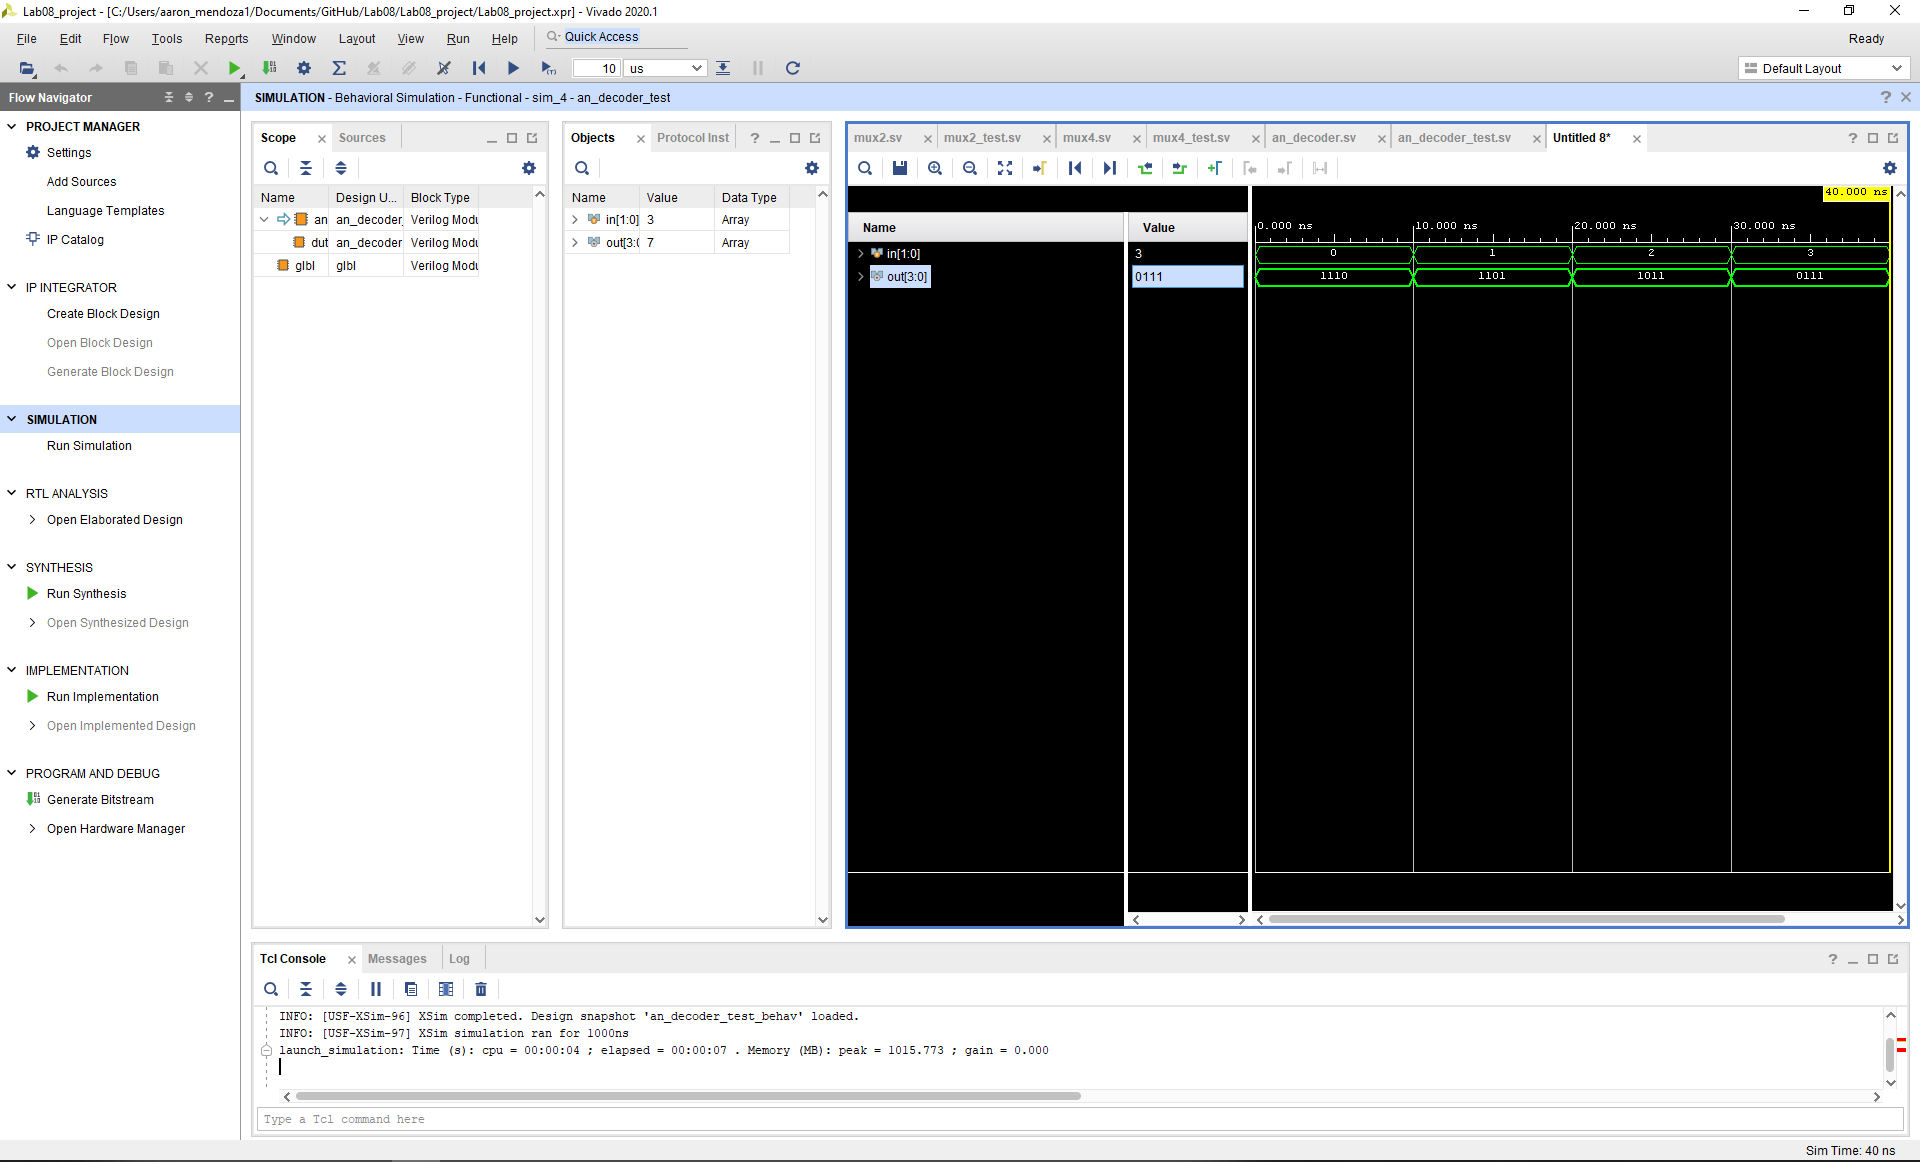
\includegraphics[width=1\textwidth,trim=19cm 15cm 0.5cm 4.5cm,clip]{an_decoder_test_screenshot}
	\caption{Anode Decoder Simulation}
	\label{fig:sim_with_table}
\end{figure}

\begin{figure}[ht]\centering
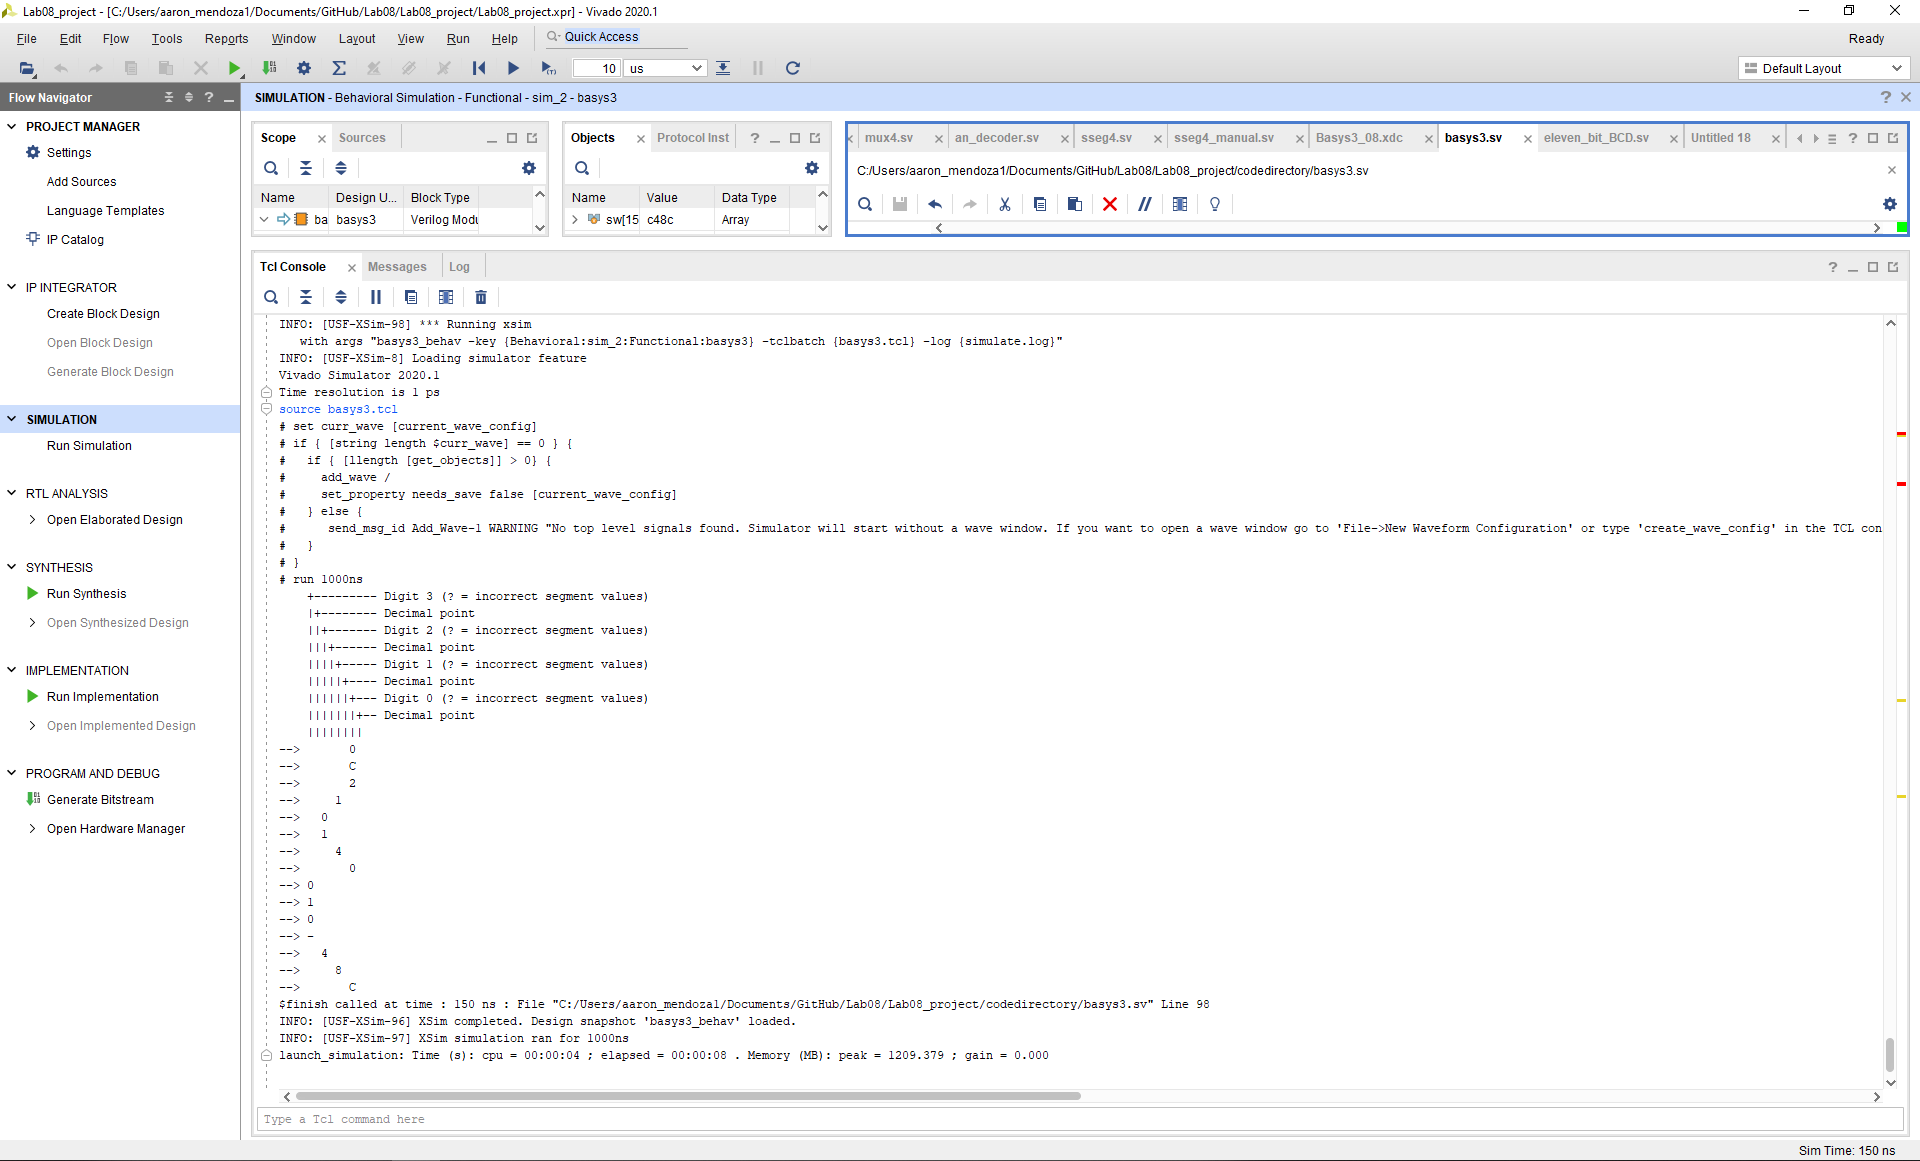
\includegraphics[width=1\textwidth,trim=7cm 3cm 15cm 10cm,clip]{top_level_sim}
	\caption{Top-Level Simulation}
	\label{fig:sim_with_table}
\end{figure}


\section*{Code}

\Verilog[firstline=22, lastline=34, caption=Add3 Module Code]{Lab08_project/codedirectory/mux2.sv}|

\Verilog[firstline=22, lastline=41, caption=Add3 Module Code]{Lab08_project/codedirectory/mux4.sv}|

\Verilog[firstline=22, lastline=35, caption=Add3 Module Code]{Lab08_project/codedirectory/an_decoder.sv}|

\Verilog[firstline=22, lastline=76, caption=Add3 Module Code]{Lab08_project/codedirectory/sseg4.sv}|

\Verilog[firstline=22, lastline=41, caption=Add3 Module Code]{Lab08_project/codedirectory/sseg4_manual.sv}|


\end{document}
